\chapter{Заключение}
 
В ходе выполнения работы был разработан плагин для движка Unity, позволяющий генерировать low poly модели деревьев во время выполнения. Плагин прост в использовании и подходит для использования в играх для мобильных устройств благодаря простоте результирующих моделей. Поддерживается генерация круглой и плоской листвы, а также хвои. Приведены примеры моделей, созданных в результате работы плагина. Была создана диаграмма классов плагина (рис. ~\ref{classDiagram}), в которую не включены особые настройки типов листвы и поля, используемые для кэширования настроек генерации.

В дальнейшем планируется усовершенствовать алгоритмы генерации для получения более разнообразных и привлекательных моделей, расширить генератор различными типами стволов (например, пальмовый или берёзовый), создать систему пресетов для генерации деревьев на основе предопределённого шаблона, а также улучшить интерфейс редактора.
 
\begin{figure}[h]
    \centering
    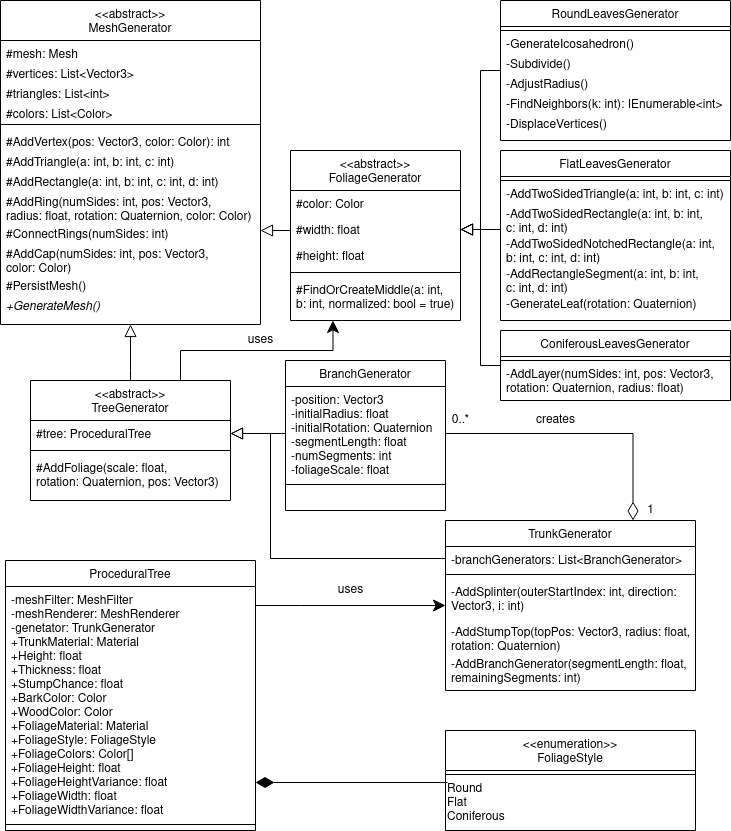
\includegraphics[width=0.8\textwidth]{classDiagram}
    \caption{Диаграмма классов разработанного плагина.}
    \label{classDiagram}
\end{figure}
